\documentclass[aspectratio=169,11pt]{beamer}
% =====================================================================
%  Le Collé — thème de présentation (même palette et mêmes notations que la fiche)
% =====================================================================
\usepackage[utf8]{inputenc}
\usepackage[T1]{fontenc}
\usepackage[sc]{mathpazo}
\usepackage[scaled=0.92]{helvet}
\usefonttheme{professionalfonts}
\usepackage{amsmath,amssymb,mathrsfs,stmaryrd}
\usepackage{microtype}
\usepackage{booktabs,array,multicol}
\usepackage[most]{tcolorbox}
\usepackage{tikz,pgfplots}
\usetikzlibrary{arrows.meta,calc,positioning,decorations.pathreplacing,shapes.misc}
\pgfplotsset{compat=1.17,trig format plots=rad}
\usepackage{tkz-tab}

% ---------- palette (identique à la fiche) ----------
\definecolor{Ink}{HTML}{1C2533}\definecolor{Bleu}{HTML}{1F3A5F}\definecolor{BleuMoyen}{HTML}{4A6A8F}
\definecolor{BleuClair}{HTML}{9DB2C9}\definecolor{Fond}{HTML}{F2F4F7}\definecolor{Ocre}{HTML}{B07A26}
\definecolor{Brique}{HTML}{A23B2A}\definecolor{Gris}{HTML}{5E6672}\definecolor{Filet}{HTML}{C5CCD6}
\definecolor{Vert}{HTML}{2E6B4F}

% ---------- notations (identiques à la fiche) ----------
\newcommand{\K}{\mathbb{K}}\newcommand{\R}{\mathbb{R}}\newcommand{\C}{\mathbb{C}}\newcommand{\Z}{\mathbb{Z}}
\newcommand{\Mn}[1]{\mathcal{M}_{n}(#1)}\newcommand{\rg}{\operatorname{rg}}\newcommand{\vect}{\operatorname{Vect}}
\newcommand{\Mat}{\operatorname{Mat}}\newcommand{\Id}{\operatorname{Id}}\newcommand{\com}{\operatorname{com}}
\newcommand{\vv}[1]{\overrightarrow{#1}}\newcommand{\ve}[1]{\vec{#1}}
\newcommand{\dt}[1]{\left|\begin{matrix}#1\end{matrix}\right|}
\DeclareRobustCommand{\HP}{{\sffamily\bfseries\scriptsize\textcolor{Brique}{[HP]}}}

% ---------- réglages beamer ----------
\setbeamertemplate{navigation symbols}{}
\setbeamersize{text margin left=0.85cm,text margin right=0.85cm}
\setbeamercolor{normal text}{fg=Ink,bg=white}
\setbeamercolor{structure}{fg=Bleu}
\setbeamercolor{alerted text}{fg=Brique}
\setbeamerfont{alerted text}{series=\bfseries}
\setbeamertemplate{itemize item}{\raisebox{0.15em}{\textcolor{Ocre}{\rule{0.38em}{0.38em}}}}
\setbeamertemplate{itemize subitem}{\textcolor{BleuMoyen}{\scriptsize\textbullet}}
\setbeamertemplate{enumerate item}{\textcolor{Bleu}{\sffamily\bfseries\insertenumlabel.}}
\setlength{\leftmargini}{1.2em}
\setbeamertemplate{blocks}[default]

% numéro de la partie courante, rappelé dans le titre et le pied de page (renvoi à la fiche)
\def\fichesec{}\def\chapnom{}
\newcommand{\chapitre}[1]{\def\chapnom{#1}}

\setbeamertemplate{frametitle}{%
  \vskip0.28cm
  \ifx\fichesec\empty\else
    \tikz[baseline=(b.base)]\node[fill=Ocre,text=white,font=\sffamily\bfseries\scriptsize,inner sep=2.5pt,rounded corners=1pt](b){\fichesec};\hspace{0.45em}%
  \fi
  {\color{Bleu}\sffamily\bfseries\Large\insertframetitle}\par
  \vskip0.06cm{\color{Filet}\rule{\linewidth}{0.5pt}}\vskip-0.2cm}

\setbeamertemplate{footline}{%
  \hbox to\paperwidth{%
    \hspace*{0.85cm}{\scriptsize\sffamily\color{Gris}Le Collé\ \ \textcolor{Filet}{|}\ \ \chapnom}\hfill
    {\scriptsize\sffamily\color{Gris}\ifx\fichesec\empty\else fiche \textbf{\color{Ocre}§\fichesec}\quad\fi\insertframenumber}\hspace*{0.85cm}}%
  \vskip0.18cm
  \hbox{\begin{tikzpicture}
    \fill[Fond] (0,0) rectangle (\paperwidth,2.2pt);
    \pgfmathsetmacro\prog{min(\insertframenumber/max(\inserttotalframenumber,1),1)}
    \fill[Ocre] (0,0) rectangle ({\prog*\paperwidth},2.2pt);
  \end{tikzpicture}}}

% ---------- encadrés : même code couleur que la fiche ----------
\tcbset{sb/.style={enhanced,arc=1pt,boxrule=0pt,left=6pt,right=6pt,top=3pt,bottom=3pt,before skip=0.14cm,after skip=0.14cm,
  fontupper=\normalsize\raggedright}}
\newcommand{\etiq}[2]{{\sffamily\bfseries\scriptsize\color{#1}\MakeUppercase{#2}}\par\vspace{2pt}}
\newtcolorbox{DEF}[1][Définition]{sb,colback=white,borderline west={2pt}{0pt}{Bleu},before upper={\etiq{Bleu}{#1}}}
\newtcolorbox{PROP}[1][Propriété]{sb,colback=Fond,borderline west={3pt}{0pt}{Bleu},before upper={\etiq{Bleu}{#1}}}
\newtcolorbox{FORM}[1][Formule]{sb,colback=white,colframe=BleuMoyen,boxrule=0.6pt,before upper={\etiq{BleuMoyen}{#1}}}
\newtcolorbox{METH}[1]{sb,colback=white,borderline north={1pt}{0pt}{Bleu},borderline south={1pt}{0pt}{Bleu},
  before upper={{\sffamily\bfseries\scriptsize\colorbox{Bleu}{\color{white}MÉTHODE}\ \color{Bleu}#1}\par\vspace{3pt}}}
\newtcolorbox{PIEGE}[1][Piège]{sb,colback=Brique!6,borderline west={2pt}{0pt}{Brique},before upper={\etiq{Brique}{#1}}}
\newtcolorbox{ASTU}[1][Astuce]{sb,colback=Ocre!8,borderline west={2pt}{0pt}{Ocre},before upper={\etiq{Ocre}{#1}}}
\newtcolorbox{HPBOX}{sb,colback=white,borderline west={2pt}{0pt}{Brique},before upper={\etiq{Brique}{Hors programme}}}
\newtcolorbox{ATOI}[1][À toi]{sb,colback=Vert!6,borderline west={2pt}{0pt}{Vert},before upper={\etiq{Vert}{#1}}}
\newtcolorbox{RETENIR}{sb,colback=Bleu!5,colframe=Bleu,boxrule=0.8pt,left=8pt,
  before upper={\etiq{Bleu}{À retenir}}}
\newtcolorbox{EX}[1][Exemple]{sb,colback=white,colframe=Filet,boxrule=0.5pt,before upper={\etiq{Gris}{#1}}}

% complément pédagogique absent du livre : étiquette pointillée
\DeclareRobustCommand{\ajout}{\tikz[baseline=(a.base)]\node[draw=Gris,dashed,text=Gris,font=\sffamily\scriptsize,inner sep=2pt,rounded corners=1pt](a){complément hors livre};}
\newcommand{\livre}[1]{{\sffamily\scriptsize\color{Gris}[livre #1]}}
\newcommand{\rep}[1]{\textcolor{Vert}{#1}}% réponse attendue de l'élève

% ---------- styles de figures (identiques au livre) ----------
\pgfplotsset{courbe/.style={axis lines=middle,axis equal image,
  axis line style={Gris,-{Stealth[length=4pt]}},
  xlabel={$x$},ylabel={$y$},ticklabel style={font=\scriptsize\sffamily,color=Gris},
  every axis x label/.style={at={(ticklabel* cs:1)},anchor=west,font=\small},
  every axis y label/.style={at={(ticklabel* cs:1)},anchor=south,font=\small},
  samples=200,smooth}}
\pgfplotsset{mini/.style={axis lines=middle,axis line style={Filet},xtick=\empty,ytick=\empty,width=3.9cm,height=3.9cm,
  xmin=-1.15,xmax=1.15,ymin=-1.15,ymax=1.15,title style={font=\footnotesize\sffamily,yshift=-0.1cm},samples=100}}
\tikzset{arcetude/.style={Bleu,line width=1.25pt},
         reste/.style={BleuClair,line width=1pt},
         tgte/.style={Ocre,line width=1pt},
         asy/.style={Gris,dashed,line width=0.7pt},
         pt/.style={circle,fill=Ink,inner sep=1.3pt},
         >={Stealth[length=5pt]}}

% ---------- diapositives de partie ----------
% \partie{num}{titre}{question guide}{liste des parties du chapitre via \rm}
\newcommand{\rmitem}[2]{\def\tmp{#1}%
  \ifx\tmp\fichesec{\color{Bleu}\bfseries #1\quad #2}\else{\color{Gris!70}#1\quad #2}\fi\par\vspace{2pt}}
\newcommand{\partie}[4]{%
  \def\fichesec{#1}\section{#2}%
  \begin{frame}[plain]
  \begin{tikzpicture}[remember picture,overlay]
    \fill[Bleu] (current page.north west) rectangle ([xshift=6.3cm]current page.south west);
    \node[anchor=north west,text=white,font=\sffamily\bfseries\fontsize{40}{40}\selectfont] at ([xshift=0.8cm,yshift=-1.2cm]current page.north west) {#1};
    \node[anchor=north west,text width=4.8cm,align=left,text=white,font=\sffamily\bfseries\Large] at ([xshift=0.8cm,yshift=-2.9cm]current page.north west) {\hyphenpenalty=10000\exhyphenpenalty=10000 #2\par};
    \node[anchor=south west,text width=4.8cm,text=white!75!Bleu,font=\sffamily\scriptsize] at ([xshift=0.8cm,yshift=0.6cm]current page.south west) {\chapnom\\fiche \textbf{§#1}};
  \end{tikzpicture}
  \hspace*{5.5cm}\begin{minipage}{8.4cm}
  {\sffamily\scriptsize\color{Ocre}\bfseries LA QUESTION}\par\vspace{2pt}
  {\large #3}\par\vspace{0.7cm}
  {\sffamily\scriptsize\color{Gris}\bfseries DANS CE CHAPITRE}\par\vspace{4pt}
  {\sffamily\small #4}
  \end{minipage}
  \end{frame}}


% ---------- exercices en séance : énoncé sur une diapositive, correction sur la suivante ----------
\newcommand{\badgeexo}[1]{\tikz[baseline=(e.base)]\node[fill=Vert,text=white,font=\sffamily\bfseries\scriptsize,inner sep=2.5pt,rounded corners=1pt](e){EXERCICE #1};\hspace{0.4em}}
\newcommand{\badgecor}[1]{\tikz[baseline=(e.base)]\node[draw=Vert,line width=0.8pt,text=Vert,font=\sffamily\bfseries\scriptsize,inner sep=2.2pt,rounded corners=1pt](e){CORRECTION #1};\hspace{0.4em}}
\newtcolorbox{ENONCE}[1][]{sb,colback=Vert!6,borderline west={3pt}{0pt}{Vert},left=9pt,top=5pt,bottom=5pt,
  before upper={{\sffamily\bfseries\scriptsize\color{Vert}À TOI\ifx\relax#1\relax\else\ \ ·\ \ \MakeUppercase{#1}\fi}\par\vspace{4pt}}}
\newtcolorbox{INDICE}{sb,colback=white,colframe=Vert!60,boxrule=0.5pt,before upper={\etiq{Vert}{Indice (si besoin)}}}
\newtcolorbox{RAIS}[1][Le raisonnement]{sb,colback=Vert!5,borderline west={2pt}{0pt}{Vert},before upper={\etiq{Vert}{#1}}}
\newtcolorbox{OUTIL}{sb,colback=Fond,borderline west={2pt}{0pt}{Bleu},before upper={\etiq{Bleu}{Propriété ou méthode utilisée}}}
\newcommand{\etape}[1]{{\sffamily\bfseries\footnotesize\color{Vert}#1}\ }
\newcommand{\objectif}[1]{\par\vspace{2pt}{\footnotesize\sffamily\color{Gris}Objectif : #1}}

\title{Le Collé --- Déterminants}

\begin{document}

% ---------------------------------------------------------------- titre
\begin{frame}[plain]
\begin{tikzpicture}[remember picture,overlay]
  \fill[Bleu] (current page.north west) rectangle (current page.south east);
  \node[anchor=north west,text=white!70!Bleu,font=\sffamily\scriptsize] at ([xshift=1cm,yshift=-1.2cm]current page.north west)
    {LE COLLÉ\ \ ·\ \ MATHÉMATIQUES PT\ \ ·\ \ CHAPITRE 2\ \ ·\ \ SUPPORT DE SÉANCE};
  \node[anchor=north west,text=white,font=\sffamily\bfseries\fontsize{26}{30}\selectfont,text width=13cm] at ([xshift=1cm,yshift=-2.1cm]current page.north west)
    {Déterminants};
  \fill[Ocre] ([xshift=1cm,yshift=-4.6cm]current page.north west) rectangle ([xshift=4cm,yshift=-4.65cm]current page.north west);
  \node[anchor=north west,text=white!80!Bleu,font=\normalsize,text width=12cm] at ([xshift=1cm,yshift=-5cm]current page.north west)
    {Présentation pour expliquer, avec quatre exercices à chercher en séance ; le \textbf{livret} pour relire, la \textbf{fiche} pour réviser.\\
     Mêmes parties (§1.1 à §1.7), mêmes notations, mêmes énoncés.};
\end{tikzpicture}
\end{frame}

% ---------------------------------------------------------------- mode d'emploi
\begin{frame}{Comment lire ce support}
\vspace{-0.15cm}
\begin{columns}[T]
\column{0.48\textwidth}
\begin{DEF}vocabulaire à connaître\end{DEF}\vspace{-9pt}
\begin{PROP}[Propriété / théorème]énoncé précis, avec ses hypothèses\end{PROP}\vspace{-9pt}
\begin{FORM}formule et conditions d'emploi\end{FORM}\vspace{-9pt}
\begin{METH}{}démarche à suivre, étape par étape\end{METH}
\column{0.48\textwidth}
\begin{PIEGE}erreur classique à éviter\end{PIEGE}\vspace{-9pt}
\begin{ASTU}technique qui fait gagner du temps\end{ASTU}\vspace{-9pt}
\begin{ATOI}question ou exercice ; correction à la diapositive suivante\end{ATOI}\vspace{-9pt}
\begin{RETENIR}l'essentiel d'une partie\end{RETENIR}
\end{columns}
{\footnotesize Même code couleur que la fiche. \ajout{} : ajout absent du livre. \ \HP{} : hors programme.
\ Le numéro ocre \tikz[baseline=(b.base)]\node[fill=Ocre,text=white,font=\sffamily\bfseries\scriptsize,inner sep=2pt](b){1.2};
\ renvoie à la partie de la fiche.}
\end{frame}

% ---------------------------------------------------------------- plan
\begin{frame}{Plan et séances}
\begin{columns}[T]
\column{0.5\textwidth}
{\sffamily\bfseries\color{Bleu}Chapitre 2 --- Déterminants}\par\vspace{4pt}
\small
1.1\quad Dimensions 2 et 3\\
1.2\quad Définition et règles de calcul \hfill{\color{Vert}Ex.~1}\\
1.3\quad Propriétés globales, endomorphismes \hfill{\color{Vert}Ex.~2}\\
1.4\quad Géométrie \hfill{\color{Vert}Ex.~3}\\
1.5\quad Quelle méthode pour quel déterminant ?\\
1.6\quad Techniques d'ordre $n$ \hfill{\color{Vert}Ex.~4}\\
{\color{Gris}1.7\quad Résultats des TD (fiche)}
\column{0.44\textwidth}
\begin{ASTU}[Découpage suggéré]
\small Séance 1 : 1.1--1.4\\ Séance 2 : 1.5--1.6, puis TD\hfill\ajout
\end{ASTU}
{\small\color{Gris}Les numéros §1.1 à §1.7 sont ceux du livret et de la fiche.}
\end{columns}
\end{frame}

% =====================================================================
%                     CHAPITRE 1 — DÉTERMINANTS
% =====================================================================
\chapitre{Chapitre 2 · Déterminants}
\def\fichesec{}
\newcommand{\rmI}{\rmitem{1.1}{Dimensions 2 et 3}\rmitem{1.2}{Définition et règles de calcul}\rmitem{1.3}{Propriétés globales, endomorphismes}
  \rmitem{1.4}{Géométrie}\rmitem{1.5}{Quelle méthode pour quel déterminant ?}\rmitem{1.6}{Techniques d'ordre $n$}\rmitem{1.7}{Résultats des TD (fiche)}}

\begin{frame}[plain]
\begin{tikzpicture}[remember picture,overlay]
  \fill[Bleu] (current page.north west) rectangle (current page.south east);
  \fill[Ocre] ([yshift=-4.2cm]current page.north west) rectangle ([yshift=-4.25cm,xshift=5cm]current page.north west);
  \node[anchor=north west,text=white!70!Bleu,font=\sffamily\small] at ([xshift=1cm,yshift=-1.6cm]current page.north west) {Chapitre 2};
  \node[anchor=north west,text=white,font=\sffamily\bfseries\fontsize{30}{32}\selectfont] at ([xshift=1cm,yshift=-2.3cm]current page.north west) {Déterminants};
  \node[anchor=north west,text width=12.5cm,text=white,font=\large] at ([xshift=1cm,yshift=-4.7cm]current page.north west)
    {Une famille de $n$ vecteurs est-elle une base ?\\[2pt]
     \normalsize\color{white!75!Bleu} Le déterminant répond par un nombre : un volume orienté, nul exactement quand les vecteurs sont liés.
     Tout le chapitre consiste à le calculer vite, et à l'interpréter.};
\end{tikzpicture}
\end{frame}

% =====================================================================
\partie{1.1}{Dimensions 2 et 3}{Comment savoir, avec un seul nombre, si deux vecteurs du plan sont colinéaires ?}{\rmI}

\begin{frame}{Deux vecteurs du plan : quand forment-ils une base ?}
\begin{columns}[T]
\column{0.5\textwidth}
\begin{ATOI}
Lesquelles de ces familles sont des bases de $\R^2$ ?
$(\ve u,\ve v)=\big((3,1),(1,2)\big)$\quad et\quad $(\ve u,\ve w)=\big((3,1),(6,2)\big)$.
\end{ATOI}
\pause
\begin{itemize}
\item $(\ve u,\ve v)$ : oui, les vecteurs ne sont pas colinéaires.
\item $(\ve u,\ve w)$ : non, $\ve w=2\ve u$.
\end{itemize}
\pause
\medskip
\textbf{Idée :} le parallélogramme construit sur deux vecteurs \alert{s'aplatit} exactement quand ils sont colinéaires.
Son aire est le bon « détecteur ».
\column{0.46\textwidth}
\centering\onslide<1->
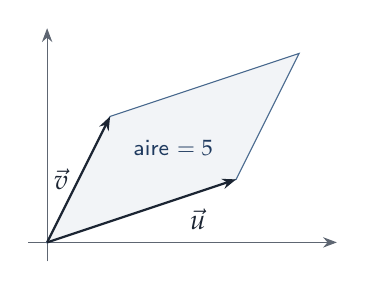
\begin{tikzpicture}[scale=0.8]
  \draw[->,Gris] (-0.3,0)--(4.6,0); \draw[->,Gris] (0,-0.3)--(0,3.4);
  \fill[Fond,draw=BleuMoyen] (0,0)--(3,1)--(4,3)--(1,2)--cycle;
  \draw[->,thick,Ink] (0,0)--(3,1) node[pos=0.7,below right]{$\ve u$};
  \draw[->,thick,Ink] (0,0)--(1,2) node[midway,left]{$\ve v$};
  \node[font=\footnotesize\sffamily,Bleu] at (2,1.5) {aire $=5$};
\end{tikzpicture}\\[4pt]
\only<3->{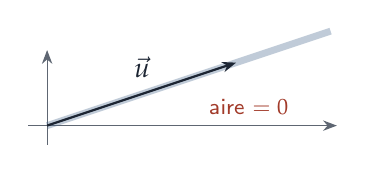
\begin{tikzpicture}[scale=0.8]
  \draw[->,Gris] (-0.3,0)--(4.6,0); \draw[->,Gris] (0,-0.3)--(0,1.2);
  \draw[BleuMoyen,line width=2.5pt,opacity=0.35] (0,0)--(4.5,1.5);
  \draw[->,thick,Ink] (0,0)--(3,1) node[pos=0.6,above left]{$\ve u$};
  \node[font=\footnotesize\sffamily,Brique] at (3.2,0.3) {aire $=0$};
\end{tikzpicture}}
\end{columns}
\end{frame}

\begin{frame}{Déterminant de deux vecteurs : une aire orientée}
\begin{columns}[c]
\column{0.55\textwidth}
\begin{FORM}[Déterminant 2×2 --- aire orientée]
$\ve u=(a,c)$, $\ve v=(b,d)$ dans une base orthonormée directe :
\[\det(\ve u,\ve v)=\dt{a&b\\c&d}=ad-bc\]\[\phantom{\det(\ve u,\ve v)}=\|\ve u\|\|\ve v\|\sin(\ve u,\ve v).\]
\end{FORM}
\pause
\begin{itemize}
\item \textbf{Valeur absolue} : aire du parallélogramme.
\item \textbf{Signe} : $+$ si l'on tourne de $\ve u$ vers $\ve v$ dans le sens direct.
\item $\det(\ve u,\ve v)=0\iff\ve u,\ve v$ colinéaires.
\end{itemize}
\column{0.4\textwidth}
\centering\onslide<1->
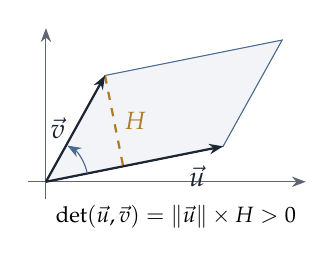
\begin{tikzpicture}[scale=0.75]
  \draw[->,Gris] (-0.3,0)--(4.4,0); \draw[->,Gris] (0,-0.3)--(0,2.6);
  \fill[Fond,draw=BleuMoyen] (0,0)--(3,0.6)--(4,2.4)--(1,1.8)--cycle;
  \draw[Ocre,dashed,thick] (1,1.8)--(1.3077,0.2615) node[midway,right,font=\small]{$H$};
  \draw[->,thick,Ink] (0,0)--(3,0.6) node[pos=0.75,below right]{$\ve u$};
  \draw[->,thick,Ink] (0,0)--(1,1.8) node[midway,left]{$\ve v$};
  \draw[->,BleuMoyen] (0.7,0.14) arc (11:60:0.7);
  \node[font=\footnotesize\sffamily] at (2.2,-0.6) {$\det(\ve u,\ve v)=\|\ve u\|\times H>0$};
\end{tikzpicture}\\[6pt]
\uncover<2->{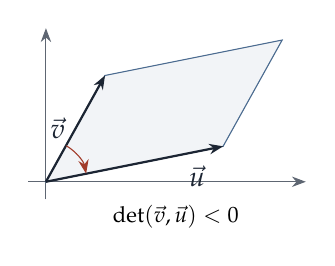
\begin{tikzpicture}[scale=0.75]
  \draw[->,Gris] (-0.3,0)--(4.4,0); \draw[->,Gris] (0,-0.3)--(0,2.6);
  \fill[Fond,draw=BleuMoyen] (0,0)--(3,0.6)--(4,2.4)--(1,1.8)--cycle;
  \draw[->,thick,Ink] (0,0)--(1,1.8) node[midway,left]{$\ve v$};
  \draw[->,thick,Ink] (0,0)--(3,0.6) node[pos=0.75,below right]{$\ve u$};
  \draw[->,Brique] (0.7*0.4903,0.7*0.8716) arc (60:11:0.7);
  \node[font=\footnotesize\sffamily] at (2.2,-0.6) {$\det(\ve v,\ve u)<0$};
\end{tikzpicture}}
\end{columns}
\end{frame}

\begin{frame}{Premier usage : inverser une matrice $2\times2$}
\begin{PROP}
Si $ad-bc\neq0$ :
\[\begin{pmatrix}a&b\\c&d\end{pmatrix}^{-1}=\dfrac1{ad-bc}\begin{pmatrix}d&-b\\-c&a\end{pmatrix}.\]
\end{PROP}
Mode d'emploi : \textbf{échanger la diagonale}, \textbf{changer les signes du reste}, \textbf{diviser par le déterminant}.
\pause
\begin{ATOI}
Inverser $A=\begin{pmatrix}3&1\\1&2\end{pmatrix}$, puis vérifier.
\end{ATOI}
\pause
\[\det A=6-1=5,\quad A^{-1}=\frac15\begin{pmatrix}2&-1\\-1&3\end{pmatrix},\quad
AA^{-1}=\frac15\begin{pmatrix}6-1&-3+3\\2-2&-1+6\end{pmatrix}=I_2.\ \ \rep{\checkmark}\]
\end{frame}

\begin{frame}{Dimension 3 : un volume orienté}
\begin{columns}[T]
\column{0.56\textwidth}
\begin{FORM}[Déterminant 3×3 --- volume orienté]
Colonnes $\ve u=(a,b,c)$, $\ve v=(d,e,f)$, $\ve w=(g,h,i)$ :
\[\dt{a&d&g\\b&e&h\\c&f&i}=a\dt{e&h\\f&i}-b\dt{d&g\\f&i}+c\dt{d&g\\e&h}.\]
\end{FORM}
\pause
\begin{itemize}
\item Produit mixte : $\det(\ve u,\ve v,\ve w)=(\ve u\wedge\ve v)\cdot\ve w$.
\item Volume $=|\det|$ = aire de base $\|\ve u\wedge\ve v\|$ $\times$ hauteur.
\item $\det=0\iff$ \textbf{coplanaires}.
\end{itemize}
\column{0.4\textwidth}
\centering\onslide<1->
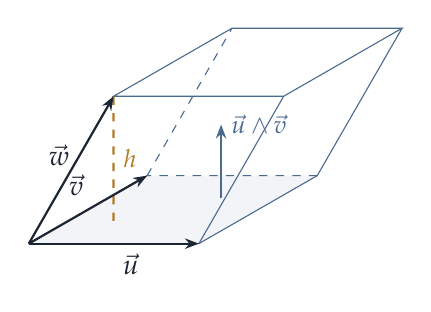
\begin{tikzpicture}[scale=0.72,x={(1cm,0cm)},y={(0.62cm,0.5cm)},z={(0cm,1cm)}]
  \coordinate (O) at (0,0,0); \coordinate (U) at (3,0,0); \coordinate (V) at (0.6,2.4,0); \coordinate (W) at (1,0.8,2.2);
  \coordinate (UV) at (3.6,2.4,0); \coordinate (UW) at (4,0.8,2.2); \coordinate (VW) at (1.6,3.2,2.2); \coordinate (UVW) at (4.6,3.2,2.2);
  \fill[Fond] (O)--(U)--(UV)--(V)--cycle;
  \draw[BleuMoyen] (O)--(U)--(UV); \draw[BleuMoyen,dashed] (UV)--(V)--(O);
  \draw[BleuMoyen] (U)--(UW) (UV)--(UVW); \draw[BleuMoyen,dashed] (V)--(VW);
  \draw[BleuMoyen] (W)--(UW)--(UVW)--(VW)--cycle;
  \draw[Ocre,dashed,thick] (1,0.8,0)--(W); \node[Ocre,font=\small,right] at (1,0.8,1.1) {$h$};
  \draw[->,thick,BleuMoyen] (2.4,1.6,0)--(2.4,1.6,1.3) node[right,font=\small]{$\ve u\wedge\ve v$};
  \draw[->,thick,Ink] (O)--(U) node[pos=0.6,below]{$\ve u$};
  \draw[->,thick,Ink] (O)--(V) node[pos=0.55,above left]{$\ve v$};
  \draw[->,thick,Ink] (O)--(W) node[pos=0.6,left]{$\ve w$};
\end{tikzpicture}
\end{columns}
\end{frame}

\begin{frame}{Calculer un $3\times3$ : à toi}
\begin{ATOI}
Calculer $D=\dt{1&0&2\\2&1&0\\0&3&1}$ de deux façons : développement selon la 1\textsuperscript{re} colonne, puis Sarrus.
\end{ATOI}
\pause
\textbf{Développement} (signes $+,-,+$) :
\[D=1\dt{1&0\\3&1}-2\dt{0&2\\3&1}+0=1\times1-2\times(0-6)=13.\]
\pause
\textbf{Sarrus} : $aei+dhc+gbf-ceg-fha-ibd=1+0+12-0-0-0=13$.\ \rep{\checkmark}
\pause
\begin{PIEGE}
Sarrus n'existe \emph{qu'en taille 3} ; au-delà : opérations et développement (§1.2).
\end{PIEGE}
\end{frame}

% =====================================================================
\partie{1.2}{Définition et règles de calcul}{En dimension $n$ on ne dessine plus : que garder de l'aire et du volume pour définir $\det$ ?}{\rmI}

\begin{frame}{Trois propriétés de l'aire orientée}
\begin{columns}[c]
\column{0.32\textwidth}\centering
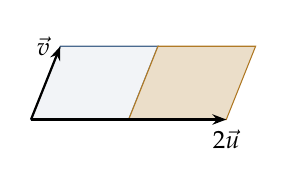
\begin{tikzpicture}[scale=0.62]
  \fill[Fond,draw=BleuMoyen] (0,0)--(2,0)--(2.6,1.5)--(0.6,1.5)--cycle;
  \fill[Ocre!25,draw=Ocre] (2,0)--(4,0)--(4.6,1.5)--(2.6,1.5)--cycle;
  \draw[->,thick] (0,0)--(4,0) node[below,font=\small]{$2\ve u$};
  \draw[->,thick] (0,0)--(0.6,1.5) node[left,font=\small]{$\ve v$};
\end{tikzpicture}\\[4pt]
\textbf{(i)} doubler un côté\\double l'aire
\column{0.32\textwidth}\centering
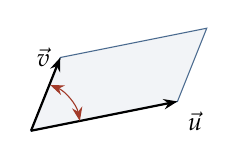
\begin{tikzpicture}[scale=0.62]
  \fill[Fond,draw=BleuMoyen] (0,0)--(3,0.6)--(3.6,2.1)--(0.6,1.5)--cycle;
  \draw[->,thick] (0,0)--(3,0.6) node[below right,font=\small]{$\ve u$};
  \draw[->,thick] (0,0)--(0.6,1.5) node[left,font=\small]{$\ve v$};
  \draw[<->,Brique] (1,0.2) arc (11:68:1);
\end{tikzpicture}\\[4pt]
\textbf{(ii)} échanger $\ve u,\ve v$\\inverse l'orientation
\column{0.32\textwidth}\centering
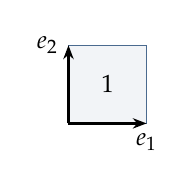
\begin{tikzpicture}[scale=0.62]
  \fill[Fond,draw=BleuMoyen] (0,0) rectangle (1.6,1.6);
  \draw[->,thick] (0,0)--(1.6,0) node[below,font=\small]{$e_1$};
  \draw[->,thick] (0,0)--(0,1.6) node[left,font=\small]{$e_2$};
  \node[font=\small] at (0.8,0.8) {$1$};
\end{tikzpicture}\\[4pt]
\textbf{(iii)} le carré unité\\a pour aire $1$
\end{columns}
\pause
\vspace{0.4cm}
\begin{center}
Ces trois propriétés \textbf{suffisent} à caractériser le déterminant, en toute dimension :\\
c'est la définition officielle.
\end{center}
\end{frame}

\begin{frame}{La définition}
\begin{DEF}[Définition --- théorème]
$\det:\Mn{\K}\to\K$ est l'\textbf{unique} application
\begin{enumerate}
\item[(i)] \textbf{linéaire par rapport à chaque colonne} (les autres fixées) :
      $\det(\dots,\lambda C_j+\mu C'_j,\dots)=\lambda\det(\dots,C_j,\dots)+\mu\det(\dots,C'_j,\dots)$ ;
\item[(ii)] \textbf{antisymétrique} : échanger deux colonnes change le signe ;
\item[(iii)] \textbf{normalisée} : $\det I_n=1$.
\end{enumerate}
\end{DEF}
\pause
\textbf{Lecture pratique :}
\begin{itemize}
\item (i) : on peut \alert{sortir un facteur} d'une colonne, et \alert{découper} une colonne en somme ;
\item (ii) : l'orientation ; \quad (iii) : le cube unité a pour volume $1$.
\end{itemize}
\end{frame}

\begin{frame}{La définition redonne la formule $ad-bc$}
Écrivons les colonnes dans la base $(e_1,e_2)$ : \quad $\det\big(ae_1+ce_2,\ be_1+de_2\big)$
\pause
\[\overset{\text{(i)}}{=}\ ab\det(e_1,e_1)+ad\det(e_1,e_2)+cb\det(e_2,e_1)+cd\det(e_2,e_2)\]
\pause
\begin{itemize}
\item (ii) : $\det(e_1,e_1)=-\det(e_1,e_1)$, donc $\det(e_1,e_1)=0$, de même $\det(e_2,e_2)=0$ ;
\item (ii) puis (iii) : $\det(e_2,e_1)=-\det(e_1,e_2)=-1$.
\end{itemize}
\pause
\[\det\big(ae_1+ce_2,\ be_1+de_2\big)=ad-bc.\qquad\rep{\text{On retrouve le §1.1.}}\]
\pause
\begin{RETENIR}
Toutes les règles de calcul qui suivent se démontrent \emph{uniquement} à partir de (i), (ii), (iii).
\end{RETENIR}
\end{frame}

\begin{frame}{Conséquences immédiates}
\begin{PROP}[Règles de calcul]
\renewcommand{\arraystretch}{1.25}
\begin{tabular}{@{}lll@{}}
$C_i\leftrightarrow C_j$ & (échange) & $\det\times(-1)$\\
$C_i\leftarrow\lambda C_i$ & (dilatation) & $\det\times\lambda$\\
$C_i\leftarrow C_i+\lambda C_j$, $j\neq i$ & (transvection) & $\det$ \textbf{inchangé}
\end{tabular}\\[3pt]
Colonne nulle, deux colonnes égales ou proportionnelles : $\det=0$.\qquad $\det(\lambda A)=\lambda^n\det A$.
\end{PROP}
\pause
\textbf{Pourquoi ?}
\begin{itemize}
\item Deux colonnes égales : les échanger ne change pas $A$ mais change le signe, donc $\det A=-\det A=0$.
\item Transvection, par (i) : $\det(\dots,C_i+\lambda C_j,\dots)=\det A+\lambda\underbrace{\det(\dots,C_j,\dots,C_j,\dots)}_{=0}$.
\item $\det(\lambda A)$ : on sort $\lambda$ de \emph{chacune} des $n$ colonnes.
\end{itemize}
\end{frame}

\begin{frame}{Développer selon une ligne ou une colonne}
\begin{PROP}[Théorème --- développement]
Pour toute ligne $i$ ou toute colonne $j$ :
\[\det A=\sum_j(-1)^{i+j}a_{i,j}\Delta_{i,j}=\sum_i(-1)^{i+j}a_{i,j}\Delta_{i,j},\]
$\Delta_{i,j}$ (\textbf{mineur}) : on supprime la ligne $i$ et la colonne $j$.
\end{PROP}
\begin{columns}[c]
\column{0.32\textwidth}\centering
Signes en damier :\\[3pt]
$\begin{pmatrix}+&-&+&\cdots\\-&+&-&\\+&-&+&\\\vdots&&&\ddots\end{pmatrix}$
\column{0.64\textwidth}
\pause
\begin{itemize}
\item On choisit la ligne ou colonne \alert{qui a le plus de zéros}.
\item Lignes et colonnes jouent le même rôle : $\det A^T=\det A$.
\item Le développement donne aussi une définition \emph{par récurrence} à partir de $ad-bc$.
\end{itemize}
\end{columns}
\end{frame}

\begin{frame}{Le cas idéal : une matrice triangulaire}
\begin{PROP}[Théorème]
Le déterminant d'une matrice triangulaire est le \textbf{produit de ses coefficients diagonaux}.
\end{PROP}
\pause
\textbf{Preuve} (récurrence) : la dernière ligne de $T$ est $(0,\dots,0,t_{n,n})$ ; on développe selon elle :
\[\det T=(-1)^{n+n}t_{n,n}\Delta_{n,n},\qquad\Delta_{n,n}\text{ triangulaire de diagonale }t_{1,1},\dots,t_{n-1,n-1}.\]
\pause
\begin{RETENIR}
Toute la stratégie de calcul en découle : \textbf{faire apparaître des zéros} par des transvections (qui ne changent pas $\det$),
jusqu'à une forme triangulaire ou une ligne à un seul coefficient.
\end{RETENIR}
\end{frame}

\begin{frame}{Méthode générale}
\begin{METH}{Calculer un déterminant}
\begin{enumerate}
\item \textbf{Regarder d'abord} la structure (tableau du §1.5) : colonnes liées ? somme constante ? ligne presque nulle ?
\item Sinon \textbf{pivot} : transvections pour créer des zéros (pivot $=1$ si possible), en notant échanges et facteurs
      sortis, jusqu'à une forme triangulaire ou une ligne/colonne à un seul coefficient ; développer selon elle.
\item Avec paramètre : \textbf{sortir les facteurs} dès qu'ils apparaissent ; ne jamais tout développer.
\end{enumerate}
\end{METH}
\end{frame}

\begin{frame}{Les pièges du calcul}
\begin{PIEGE}[Pièges]
\begin{itemize}
\item $\det(A+B)\neq\det A+\det B$ ;\quad $\det(\lambda A)\neq\lambda\det A$.
\item Transvection : la colonne modifiée garde le coefficient $1$ ($C_i\leftarrow2C_i+C_j$ multiplie par $2$).
\item Opérations successives : chacune agit sur la matrice \emph{déjà} modifiée.
\item Oublier le signe $(-1)^{i+j}$ du développement.
\end{itemize}
\end{PIEGE}
\end{frame}

\begin{frame}{Exemple : regarder avant de calculer}
\begin{columns}[c]
\column{0.4\textwidth}
\[D=\dt{1&2&3&4\\4&1&2&3\\3&4&1&2\\2&3&4&1}\]
\column{0.56\textwidth}
\begin{ATOI}
Avant tout calcul : que remarques-tu sur les lignes ?
\end{ATOI}
\end{columns}
\pause
\rep{Chaque ligne a pour somme $10$.} \ D'où : $C_1\leftarrow C_1+C_2+C_3+C_4$, puis on sort $10$ :
\pause
\[D=10\dt{1&2&3&4\\1&1&2&3\\1&4&1&2\\1&3&4&1}\overset{L_i-L_1}{=}10\dt{1&2&3&4\\0&-1&-1&-1\\0&2&-2&-2\\0&1&1&-3}
=10\dt{-1&-1&-1\\2&-2&-2\\1&1&-3}\]
\pause
$C_2-C_1$, $C_3-C_1$ : \ $\dt{-1&0&0\\2&-4&-4\\1&0&-4}=-1\times16=-16$, \ donc \ $\boxed{D=-160}$.
\end{frame}

% ---------------------------------------------------------------- EXERCICE D1
\begin{frame}{\badgeexo{1}Les règles de calcul en action}
\begin{ENONCE}[5 min]
\begin{enumerate}
\item Calculer $\dt{1&2&1\\2&5&3\\-1&1&4}$ par opérations sur les lignes.
\item Sans aucun calcul : que vaut $\dt{1&2&3\\4&5&6\\7&8&9}$ ?
\item $A\in\mathcal M_3(\R)$ avec $\det A=5$. Que vaut $\det(2A)$ ? et $\det(-A^T)$ ?
\end{enumerate}
\objectif{transvections, colonnes liées, $\det(\lambda A)=\lambda^n\det A$. Indice pour 2 : comparer $C_1+C_3$ et $C_2$.}
\end{ENONCE}
\end{frame}

\begin{frame}{\badgecor{1}Les règles de calcul en action}
\begin{columns}[T]
\column{0.38\textwidth}
\begin{RAIS}
Créer des zéros par transvections (déterminant inchangé), repérer une relation entre colonnes, compter les facteurs sortis.
\end{RAIS}
\begin{OUTIL}
Règles de calcul (§1.2) ; colonnes liées $\Rightarrow\det=0$.
\end{OUTIL}
\column{0.59\textwidth}
\etape{1.} $L_2\leftarrow L_2-2L_1$, $L_3\leftarrow L_3+L_1$ :
$\dt{1&2&1\\0&1&1\\0&3&5}=1\times(5-3)=2$.\\[3pt]
\pause
\etape{2.} $C_1+C_3=2C_2$ : colonnes liées, le déterminant est \textbf{nul}.\\[3pt]
\pause
\etape{3.} $\det(2A)=2^3\cdot5=40$ ; \ $\det(-A^T)=(-1)^3\det A=-5$.
\end{columns}
{\small\color{Brique}\textbf{Piège :} $\det(2A)\neq2\det A$, les trois colonnes sont multipliées par $2$.}
\end{frame}

% =====================================================================
\partie{1.3}{Propriétés globales, endomorphismes}{Que dit le déterminant d'une matrice, d'un produit, d'un endomorphisme ?}{\rmI}

\begin{frame}{Le théorème fondamental}
\begin{PROP}[Théorème fondamental]
$A$ inversible $\iff\det A\neq0\iff$ colonnes libres.\\[3pt]
$\det(AB)=\det A\det B$ ;\quad $\det A^{-1}=\dfrac1{\det A}$ ;\quad $\det A^T=\det A$ ;\quad $\det(PBP^{-1})=\det B$.
\end{PROP}
\pause
\textbf{Idée de preuve.}
\begin{itemize}
\item Colonnes liées : $C_i=\sum_{j\neq i}\lambda_jC_j$ ; la transvection $C_i\leftarrow C_i-\sum\lambda_jC_j$ crée une colonne nulle : $\det A=0$.
\item $A$ inversible : $\det A\det A^{-1}=\det I_n=1$, donc $\det A\neq0$.
\end{itemize}
\pause
\begin{PIEGE}
Le déterminant est \emph{multiplicatif}, pas additif : il passe aux produits, inverses, transposées, jamais aux sommes.
\end{PIEGE}
\end{frame}

\begin{frame}{Des questions sans aucun coefficient}
\begin{METH}{Question sans coefficients}
Une relation entre matrices $\Rightarrow$ on applique $\det$ aux deux membres.
\end{METH}
\begin{ATOI}
$A\in\Mn{\R}$ vérifie $A^2=-I_n$. Que peut-on dire de $n$ ?
\end{ATOI}
\pause
$(\det A)^2=\det(-I_n)=(-1)^n$. Un carré réel est $\geq0$, donc \rep{$n$ est pair}.\quad
\alert{Faux dans $\C$} : $A=iI_n$.
\pause
\begin{ATOI}
$A$ antisymétrique ($A^T=-A$) d'ordre $n$ impair : $\det A$ ?
\end{ATOI}
\pause
$\det A=\det A^T=\det(-A)=(-1)^n\det A=-\det A$, donc \rep{$\det A=0$}.
\pause\par
\textbf{Autre cas :} $A^2=A$, $A\neq I_n$ : $\det A\in\{0,1\}$, et $\det A=1$ forcerait $A=I_n$ ; donc $\det A=0$.
\end{frame}

\begin{frame}{Déterminant d'une famille, d'un endomorphisme}
\begin{DEF}
$\det_{\mathcal B}(u_1,\dots,u_n)$ : déterminant des coordonnées des $u_j$ dans la base $\mathcal B$.\\
$\det f=\det\Mat_{\mathcal B}(f)$ \ --- \ indépendant de $\mathcal B$ (matrices semblables).
\end{DEF}
\begin{PROP}
$(u_1,\dots,u_n)$ base de $E$ ($\dim E=n$) $\iff\det_{\mathcal B}(u_j)\neq0$ ;\quad $f$ automorphisme $\iff\det f\neq0$.\\
$\det(f\circ g)=\det f\det g$,\quad $\det(\lambda f)=\lambda^n\det f$,\quad $\det f^{-1}=\frac1{\det f}$.
\end{PROP}
\pause
\begin{EX}
$(1,\,1+X,\,\dots,\,1+X+\dots+X^n)$ : base de $\R_n[X]$ (triangulaire, diagonale de $1$).\\
Dérivation $D$ sur $\R_n[X]$ : diagonale nulle, $\det D=0$ : non bijective.
\end{EX}
\end{frame}

\begin{frame}{Le bon réflexe : la base adaptée}
\begin{columns}[c]
\column{0.58\textwidth}
\begin{PROP}[Projecteurs, symétries]
Projecteur $p$ : $\det p=1$ si $p=\Id$, $0$ sinon.\\[2pt]
Symétrie $s$ :\ \ $\det s=(-1)^{\dim\mathrm{Ker}(s+\Id)}=(-1)^{n-\rg(s+\Id)}$.
\end{PROP}
\pause
\textbf{Pourquoi :} dans une base adaptée,
\[\Mat p=\mathrm{diag}(I_r,0),\qquad\Mat s=\mathrm{diag}(I_r,-I_{n-r}).\]
\pause
\begin{RETENIR}
Endomorphisme défini géométriquement $\Rightarrow$ \textbf{base adaptée}, jamais la base canonique.
\end{RETENIR}
\column{0.38\textwidth}\centering\onslide<1->
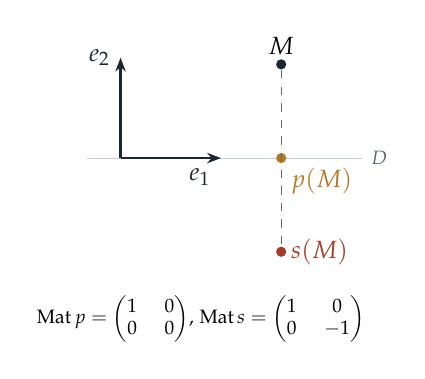
\begin{tikzpicture}[scale=0.85]
  \draw[Filet] (-0.5,0)--(3.6,0) node[right,font=\scriptsize,Gris]{$D$};
  \draw[->,thick,Ink] (0,0)--(1.5,0) node[below left,font=\small]{$e_1$};
  \draw[->,thick,Ink] (0,0)--(0,1.5) node[left,font=\small]{$e_2$};
  \node[pt] (M) at (2.4,1.4) {}; \node[font=\small,above] at (M) {$M$};
  \node[pt,fill=Ocre] (P) at (2.4,0) {}; \node[font=\small,below right,Ocre] at (P) {$p(M)$};
  \node[pt,fill=Brique] (S) at (2.4,-1.4) {}; \node[font=\small,right,Brique] at (S) {$s(M)$};
  \draw[dashed,Gris] (M)--(S);
  \node[font=\scriptsize,align=left] at (1.2,-2.4) {$\Mat p=\begin{pmatrix}1&0\\0&0\end{pmatrix}$,\ $\Mat s=\begin{pmatrix}1&0\\0&-1\end{pmatrix}$};
\end{tikzpicture}\\
{\scriptsize projection sur $D$ et réflexion d'axe $D$ :\\ $\det p=0$, $\det s=-1$}
\end{columns}
\end{frame}

\begin{frame}{Base adaptée : deux exemples de TD}
\begin{EX}[$f:M\mapsto AM$ sur $\mathcal M_2(\R)$]
Base $(E_{11},E_{21},E_{12},E_{22})$ : on agit colonne par colonne, donc $\Mat f=\mathrm{diag}(A,A)$ et
$\det f=(\det A)^2$ \ (en taille $n$ : $(\det A)^n$).
\end{EX}
\pause
\begin{FORM}[Similitudes \HP{} --- TD 8]
$\C$ vu comme $\R$-espace vectoriel, base $(1,i)$, $a=\alpha+i\beta$ :
\begin{itemize}
\item $z\mapsto az$ : $\begin{pmatrix}\alpha&-\beta\\\beta&\alpha\end{pmatrix}$, $\det=|a|^2$, $\mathrm{tr}=2\,\mathrm{Re}\,a$ ;
      symétrie $\iff a=\pm1$ ; $|a|=1$ : rotation d'angle $\arg a$.
\item $z\mapsto a\bar z$ : $\begin{pmatrix}\alpha&\beta\\\beta&-\alpha\end{pmatrix}$, $\det=-|a|^2$ ; réflexion si $|a|=1$.
\end{itemize}
$\det f>0$ : orientation conservée ; $<0$ : renversée.
\end{FORM}
\end{frame}

% ---------------------------------------------------------------- EXERCICE D2
\begin{frame}{\badgeexo{2}Déterminant d'un endomorphisme}
\begin{ENONCE}[6 min]
Calculer le déterminant des endomorphismes suivants, en choisissant une base adaptée.
\begin{enumerate}
\item $T:\mathcal M_2(\R)\to\mathcal M_2(\R)$, $M\mapsto M^T$.
\item $g:\R_2[X]\to\R_2[X]$, $P\mapsto P(X+1)$. Est-ce un automorphisme ?
\end{enumerate}
\objectif{ne jamais calculer dans une base mal choisie.}
\end{ENONCE}
\pause
\begin{INDICE}
1 : matrices symétriques, matrices antisymétriques. \quad 2 : images de $1$, $X$, $X^2$.
\end{INDICE}
\end{frame}

\begin{frame}{\badgecor{2}Déterminant d'un endomorphisme}
\begin{columns}[T]
\column{0.38\textwidth}
\begin{RAIS}
$\det f$ ne dépend pas de la base : on prend celle où la matrice est diagonale ou triangulaire.
\end{RAIS}
\begin{OUTIL}
$\det f=\det\Mat_{\mathcal B}(f)$ ; matrice triangulaire.
\end{OUTIL}
\column{0.59\textwidth}
\etape{1.} Base $\big(E_{11},E_{22},E_{12}+E_{21}\big)$ (symétriques, $T=\Id$) complétée par $E_{12}-E_{21}$ (antisymétrique, $T=-\Id$) :
$\Mat(T)=\mathrm{diag}(1,1,1,-1)$, \ $\det T=-1$.\\[3pt]
\pause
\etape{2.} $g(1)=1$, $g(X)=1+X$, $g(X^2)=1+2X+X^2$ : dans $(1,X,X^2)$,
$\Mat(g)=\begin{pmatrix}1&1&1\\0&1&2\\0&0&1\end{pmatrix}$, triangulaire : $\det g=1\neq0$, \textbf{automorphisme}.
\end{columns}
\end{frame}

\begin{frame}{Pour aller plus loin : la comatrice \HP}
\begin{HPBOX}
$\com(A)=\big((-1)^{i+j}\Delta_{i,j}\big)$ \ (matrice des cofacteurs). Pour toute $A$ :
\[A\,\com(A)^T=\com(A)^TA=\det(A)\,I_n,\]
donc, si $\det A\neq0$ :\quad $A^{-1}=\dfrac1{\det A}\com(A)^T$.
\end{HPBOX}
\pause
\textbf{Pourquoi :} le coefficient $(i,i)$ de $A\,\com(A)^T$ est le développement de $\det A$ selon la ligne $i$ ; le
coefficient $(k,i)$, $k\neq i$, développe une matrice à deux lignes égales : $0$.
\pause
\begin{itemize}
\item En taille 2 : la formule du §1.1 ;\quad $\det\com(A)=(\det A)^{n-1}$.
\item $A$ entière : $A^{-1}$ entière $\iff\det A=\pm1$.
\end{itemize}
\begin{PIEGE}
\emph{Transposer} la comatrice ; mettre le signe $(-1)^{i+j}$ sur chaque cofacteur.
\end{PIEGE}
\end{frame}

% =====================================================================
\partie{1.4}{Géométrie}{Comment traduire « alignés », « coplanaires », « aire », « distance » par un déterminant ?}{\rmI}

\begin{frame}{Le dictionnaire géométrique}
\begin{FORM}[Traductions (base orthonormée)]
\renewcommand{\arraystretch}{1.35}
\begin{tabular}{@{}ll@{}}
$A,B,C$ alignés & $\det(\vv{AB},\vv{AC})=0$\\
$M(x,y)\in(BC)$ & $\dt{1&1&1\\x&b&c\\y&b'&c'}=0$\\
$M\in(ABC)$ & $\det(\vv{AM},\vv{AB},\vv{AC})=0$\\
aire du triangle $ABC$ & $\frac12|\det(\vv{AB},\vv{AC})|$\\
volume du tétraèdre $ABCD$ & $\frac16|\det(\vv{AB},\vv{AC},\vv{AD})|$\\
$A+\vect\ve u$, $C+\vect\ve v$ coplanaires & $\det(\vv{AC},\ve u,\ve v)=0$
\end{tabular}\\[2pt]
{\small Pour $(BC)$, avec $B(b,b')$, $C(c,c')$ : $C_1-C_2$, $C_3-C_2$ donnent $-\det(\vv{BM},\vv{BC})$.}
\end{FORM}
\end{frame}

\begin{frame}{Le dictionnaire en action}
\begin{ATOI}
$A(1,2)$, $B(2,-2)$, $C(3,1)$ : aire du triangle ? Équation de $(AB)$ ?
\end{ATOI}
\pause
\begin{itemize}
\item $\vv{AB}=(1,-4)$, $\vv{AC}=(2,-1)$ :\quad $\det(\vv{AB},\vv{AC})=\dt{1&2\\-4&-1}=7$ :\quad \rep{aire $\frac72$}.
\pause
\item $M(x,y)\in(AB)\iff\dt{1&x-1\\-4&y-2}=0\iff$ \rep{$y=-4x+6$}.
\end{itemize}
\pause
\begin{ASTU}
On écrit toujours la condition sous la forme « $\det=0$ » : l'équation sort directement, sans calculer de pente.
\end{ASTU}
\end{frame}

\begin{frame}{Distance de deux droites de l'espace}
\begin{columns}[c]
\column{0.5\textwidth}
\begin{FORM}[Distance --- TD 2]
$\mathcal D_1=A+\vect\ve u$, $\mathcal D_2=C+\vect\ve v$ non parallèles :
\[d(\mathcal D_1,\mathcal D_2)=\frac{|\det(\vv{AC},\ve u,\ve v)|}{\|\ve u\wedge\ve v\|}.\]
\end{FORM}
\pause
\textbf{Lecture :} $|\det(\vv{AC},\ve u,\ve v)|$ est le volume du parallélépipède de base $\|\ve u\wedge\ve v\|$ et de
hauteur $d$ : \alert{volume / base}.
\pause\par\smallskip
\textbf{Perpendiculaire commune :} $H=A+s\ve u$, $K=C+r\ve v$ avec $\vv{HK}\cdot\ve u=\vv{HK}\cdot\ve v=0$.\\
Sécantes $\iff d=0$.
\column{0.47\textwidth}\centering\onslide<1->
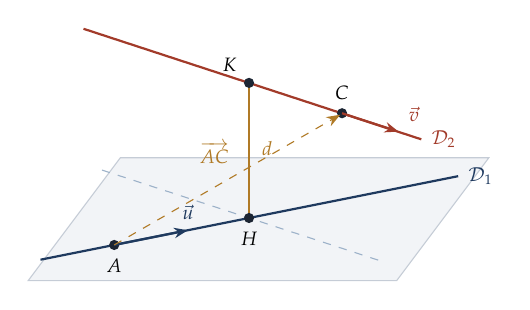
\begin{tikzpicture}[scale=0.78]
\fill[Fond] (0,0)--(6,0)--(7.5,2)--(1.5,2)--cycle; \draw[Filet] (0,0)--(6,0)--(7.5,2)--(1.5,2)--cycle;
\draw[Bleu,thick] (0.2,0.34)--(7.0,1.70) node[right,font=\scriptsize]{$\mathcal D_1$};
\draw[BleuClair,dashed] (1.2,1.8)--(5.8,0.3);
\draw[Brique,thick] (0.9,4.1)--(6.4,2.3) node[right,font=\scriptsize]{$\mathcal D_2$};
\draw[Ocre,thick] (3.595,1.019)--(3.595,3.219);
\node[pt] at (3.595,1.019) {}; \node[font=\scriptsize,anchor=north] at (3.595,0.95) {$H$};
\node[pt] at (3.595,3.219) {}; \node[font=\scriptsize,anchor=south east] at (3.55,3.25) {$K$};
\node[font=\scriptsize,Ocre,anchor=west] at (3.65,2.15) {$d$};
\node[pt] at (1.4,0.58) {}; \node[font=\scriptsize,anchor=north] at (1.4,0.52) {$A$};
\draw[->,Bleu,thick] (1.4,0.58)--(2.6,0.82) node[above,font=\scriptsize]{$\ve u$};
\node[pt] at (5.11,2.725) {}; \node[font=\scriptsize,anchor=south] at (5.11,2.78) {$C$};
\draw[->,Brique,thick] (5.11,2.725)--(6.03,2.425) node[above right,font=\scriptsize]{$\ve v$};
\draw[->,Ocre,dashed] (1.4,0.58)--(5.08,2.70) node[pos=0.55,above left,font=\scriptsize]{$\vv{AC}$};
\end{tikzpicture}\\
{\scriptsize Plan gris : contient $\mathcal D_1$, parallèle à $\mathcal D_2$.}
\end{columns}
\end{frame}

% ---------------------------------------------------------------- EXERCICE D3
\begin{frame}{\badgeexo{3}Coplanaires ? Quel volume ?}
\begin{ENONCE}[5 min]
Dans l'espace muni d'un repère orthonormé, $A(1,2,0)$, $B(2,3,1)$, $C(0,1,1)$, $D(1,1,2)$.
\begin{enumerate}
\item Les quatre points sont-ils coplanaires ?
\item Calculer le volume du tétraèdre $ABCD$.
\end{enumerate}
\objectif{le dictionnaire géométrique du §1.4.}
\end{ENONCE}
\end{frame}

\begin{frame}{\badgecor{3}Coplanaires ? Quel volume ?}
\begin{columns}[T]
\column{0.38\textwidth}
\begin{RAIS}
Coplanaires $\iff\det(\vv{AB},\vv{AC},\vv{AD})=0$ ; sinon, ce déterminant est le volume orienté du parallélépipède, le tétraèdre
en vaut le sixième.
\end{RAIS}
\column{0.59\textwidth}
\etape{1.} $\vv{AB}=(1,1,1)$, $\vv{AC}=(-1,-1,1)$, $\vv{AD}=(0,-1,2)$. Avec $C_2\leftarrow C_2+C_1$ :
\[\dt{1&-1&0\\1&-1&-1\\1&1&2}=\dt{1&0&0\\1&0&-1\\1&2&2}=2.\]
Non nul : \textbf{non coplanaires}.\\[3pt]
\pause
\etape{2.} $\mathcal V=\frac16|2|=\frac13$.
\end{columns}
\end{frame}

% =====================================================================
\partie{1.5}{Quelle méthode pour quel déterminant ?}{Face à un déterminant d'ordre $n$, comment choisir la bonne technique avant de calculer ?}{\rmI}

\begin{frame}{La carte des méthodes}
\footnotesize
\renewcommand{\arraystretch}{1.12}
\begin{tabular}{@{}>{\raggedright}p{0.42\linewidth}>{\raggedright\arraybackslash}p{0.48\linewidth}r@{}}
\toprule
\textsf{\footnotesize Je vois\dots} & \textsf{\footnotesize Je fais\dots} & \\\midrule
colonnes combinaisons de $\leq2$ vecteurs ($i+j$\dots) & $\det=0$ ($n\geq3$) & \\
même somme sur chaque ligne & $C_1\leftarrow\sum C_j$, sortir la somme, $L_i-L_1$ & \textcolor{Ocre}{1.6}\\
$a_{i,j}$ formule ($\max$, $|i-j|$, $a^{|i-j|}$) & $C_k-C_{k-1}$ (ou $-aC_{k-1}$), $k=n\to2$ & \textcolor{Ocre}{1.6}\\
ligne/colonne à 1 coefficient & développer selon elle & \textcolor{Ocre}{1.2}\\
lettres X, Z, N & développer ; permuter lignes \emph{et} colonnes & \textcolor{Ocre}{1.6}\\
puissances $1,x,x^2,\dots$ & Vandermonde / polynôme en $x$ & \textcolor{Ocre}{1.6}\\
tridiagonal & récurrence d'ordre 2 & \textcolor{Ocre}{1.6}\\
$a$ au-dessus, $b$ au-dessous, constante ajoutée & fonction affine ; $a=b$ par dérivée & \textcolor{Ocre}{1.6}\\
relation entre matrices & $\det(AB)$, $\det(\lambda A)$, $\det A^T$ & \textcolor{Ocre}{1.3}\\
endomorphisme géométrique & base adaptée & \textcolor{Ocre}{1.3}\\
\bottomrule
\end{tabular}\\[4pt]
{\footnotesize\color{Gris}Ce tableau est le §1.5 de la fiche : on y revient au début de chaque exercice.}
\end{frame}

% =====================================================================
\partie{1.6}{Techniques d'ordre $n$}{Comment calculer un déterminant dont la taille $n$ est une lettre ?}{\rmI}

\begin{frame}{Somme constante}
\begin{columns}[c]
\column{0.36\textwidth}
\[D_n(a,b)=\dt{a&b&\cdots&b\\b&a&\ddots&\vdots\\\vdots&\ddots&\ddots&b\\b&\cdots&b&a}\]
\column{0.6\textwidth}
\pause
\begin{enumerate}
\item Chaque ligne a pour somme $a+(n-1)b$ : $C_1\leftarrow C_1+\dots+C_n$, on sort ce facteur.
\item $L_i\leftarrow L_i-L_1$ ($i\geq2$) : triangulaire de diagonale $(1,a-b,\dots,a-b)$.
\end{enumerate}
\end{columns}
\pause
\begin{FORM}
\[D_n(a,b)=\big(a+(n-1)b\big)(a-b)^{n-1}.\]
Inversible $\iff a\neq b$ et $a+(n-1)b\neq0$ \ ($n\geq2$). \quad C'est la matrice $(a-b)I_n+bJ$ du TD 6.
\end{FORM}
\end{frame}

\begin{frame}{Formule en $i,j$ : les différences successives}
\begin{METH}{Différences successives}
$C_k\leftarrow C_k-C_{k-1}$ pour $k=n,n-1,\dots,2$ (\textbf{depuis la fin} : chaque opération utilise une colonne intacte).
Nouveau coefficient : distinguer $i<k$ et $i\geq k$.
\end{METH}
\pause
\textbf{Exemple} $a_{i,j}=\max(i,j)$, $n=4$ :
\[\begin{pmatrix}1&2&3&4\\2&2&3&4\\3&3&3&4\\4&4&4&4\end{pmatrix}\ \longrightarrow\
\begin{pmatrix}1&1&1&1\\2&0&1&1\\3&0&0&1\\4&0&0&0\end{pmatrix}\]
\pause
Dernière ligne $(n,0,\dots,0)$ : on développe, le mineur est triangulaire à diagonale de $1$ :
\[\det\big(\max(i,j)\big)=(-1)^{n+1}n\qquad(\text{ici }-4).\]
\end{frame}

\begin{frame}{Différences successives : résultats à connaître}
\begin{FORM}[Résultats]
\renewcommand{\arraystretch}{1.3}
\begin{tabular}{@{}ll@{}}
$\det\big(\max(i,j)\big)=(-1)^{n+1}n$ & dernière ligne $(n,0,\dots,0)$\\
$\det\big(|i-j|\big)=(-1)^{n-1}(n-1)2^{n-2}$ & colonnes, puis $L_i-L_{i-1}$, puis $C_1+\frac12\sum_{k\geq2}C_k$\\
$\det\big(a^{|i-j|}\big)=(1-a^2)^{n-1}$ & avec $C_k-aC_{k-1}$
\end{tabular}
\end{FORM}
\pause
\begin{ATOI}[Contrôle]
Vérifier la formule $|i-j|$ pour $n=2$, $n=3$.
\end{ATOI}
\pause
\[n=2:\ \dt{0&1\\1&0}=-1=(-1)^1\cdot1\cdot2^0\ \rep{\checkmark}\quad
n=3:\ \dt{0&1&2\\1&0&1\\2&1&0}=4=(-1)^2\cdot2\cdot2\ \rep{\checkmark}\]
\end{frame}

% ---------------------------------------------------------------- EXERCICE D4
\begin{frame}{\badgeexo{4}La matrice $\min(i,j)$}
\begin{ENONCE}[5 min]
Pour $n\geq1$, calculer $\Delta_n=\det\big(\min(i,j)\big)_{1\leq i,j\leq n}$, par exemple
$\Delta_4=\dt{1&1&1&1\\1&2&2&2\\1&2&3&3\\1&2&3&4}$.
\objectif{les différences successives, dans le bon ordre.}
\end{ENONCE}
\pause
\begin{INDICE}
Que vaut la ligne $L_i-L_{i-1}$ ? Par quelle ligne commencer ?
\end{INDICE}
\end{frame}

\begin{frame}{\badgecor{4}La matrice $\min(i,j)$}
\begin{columns}[T]
\column{0.38\textwidth}
\begin{RAIS}
Deux lignes consécutives ne diffèrent que sur la fin : leurs différences font apparaître une matrice triangulaire.
\end{RAIS}
\begin{OUTIL}
Différences successives (§1.6) ; matrice triangulaire.
\end{OUTIL}
\column{0.59\textwidth}
\etape{1.} $L_i-L_{i-1}=(0,\dots,0,1,\dots,1)$, le premier $1$ en colonne $i$.\\[3pt]
\etape{2.} On fait $L_n\leftarrow L_n-L_{n-1}$, puis $L_{n-1}\leftarrow L_{n-1}-L_{n-2}$, \dots, $L_2\leftarrow L_2-L_1$ :
\emph{chaque opération utilise une ligne pas encore modifiée}.\\[3pt]
\pause
\etape{3.} La matrice obtenue est triangulaire supérieure, de diagonale $(1,\dots,1)$ : $\Delta_n=1$.
\end{columns}
\begin{PIEGE}
Commencer par $L_2-L_1$ puis $L_3-L_2$ utiliserait une ligne \emph{déjà modifiée}.
\end{PIEGE}
\end{frame}

\begin{frame}{Déterminants creux : X, Z, N}
\begin{columns}[c]
\column{0.3\textwidth}\centering
$\begin{pmatrix}a&&&b\\&a&b&\\&b&a&\\b&&&a\end{pmatrix}$\\[2pt]{\scriptsize « X » d'ordre $4$}
\column{0.66\textwidth}
\begin{ASTU}[Astuces]
\begin{itemize}
\item Permuter lignes et colonnes par la \emph{même} permutation ne change pas $\det$ ($P^{-1}AP$) : on regroupe en blocs.
\item Inverser l'ordre de $m$ lignes : $\lfloor m/2\rfloor$ échanges.
\item Ligne à un seul coefficient : la sortir, puis s'en servir de pivot.
\end{itemize}
\end{ASTU}
\end{columns}
\pause
\textbf{X d'ordre $2n$ :} réordonner selon $1,2n,2,2n-1,\dots$ : $n$ blocs $\begin{pmatrix}a&b\\b&a\end{pmatrix}$, d'où
$(a^2-b^2)^n$.
\end{frame}

\begin{frame}{Déterminants creux : résultats}
\begin{FORM}[Résultats --- TD 4, TD 9]
X d'ordre $2n$ : $(a^2-b^2)^n$ ; ordre $2n+1$ (centre $a$) : $a(a^2-b^2)^n$.\\
Z d'ordre $n$ : $(-1)^{\lfloor\frac{n-2}2\rfloor}b_2\cdots b_{n-1}(a_1c_n-a_nc_1)$ ;\quad
N ($b_j$ sur la diagonale) : $b_2\cdots b_{n-1}(a_1c_n-a_nc_1)$.
\end{FORM}
\pause
\begin{PIEGE}
Le signe de l'anti-diagonale : le $b$ de la première ligne est en position $(1,2n)$, de signe $(-1)^{2n+1}=-1$.
Une erreur de signe donnerait $(a^2+b^2)^n$, faux dès $n=1$.
\end{PIEGE}
\pause
\begin{RETENIR}
Toujours tester la formule finale sur $n=3$ ou $4$.
\end{RETENIR}
\end{frame}

\begin{frame}{Vandermonde}
\begin{FORM}[Théorème --- Vandermonde]
\[V(x_1,\dots,x_n)=\det\big(x_j^{\,i-1}\big)=\dt{1&1&\cdots&1\\x_1&x_2&\cdots&x_n\\\vdots&&&\vdots\\x_1^{n-1}&x_2^{n-1}&\cdots&x_n^{n-1}}=\prod_{i<j}(x_j-x_i),\]
non nul $\iff$ les $x_i$ sont distincts.\quad $n=3$ : $(b-a)(c-a)(c-b)$.
\end{FORM}
\pause
\textbf{D'où vient le produit ?} Regardons la dernière variable comme une inconnue $x$ : c'est la méthode suivante.
\end{frame}

\begin{frame}{Voir un déterminant comme un polynôme}
\begin{METH}{Polynôme en $x$}
$x$ dans une seule colonne $\Rightarrow$ développer selon elle : $P(x)$ est un polynôme.
\begin{enumerate}
\item Coefficient dominant = cofacteur de la plus haute puissance.
\item Racines évidentes : valeurs rendant deux colonnes égales.
\item Autant de racines que le degré $\Rightarrow P=$ coeff.\ dominant $\times\prod(x-\text{racine})$.
\end{enumerate}
\end{METH}
\pause
\textbf{Exemple :} $P(x)=\dt{1&1&1\\a&b&x\\a^2&b^2&x^2}$ ($a\neq b$).
\pause
\begin{itemize}
\item Degré $\leq2$, coefficient de $x^2$ : $\dt{1&1\\a&b}=b-a$ ;\quad $P(a)=P(b)=0$ (colonnes égales).
\end{itemize}
\pause
\[P(x)=(b-a)(x-a)(x-b)\qquad\Rightarrow\qquad V(a,b,c)=(b-a)(c-a)(c-b).\]
\end{frame}

\begin{frame}{Polynôme en $x$ : deux précautions}
\begin{PIEGE}[Piège : un terme manquant]
Une puissance manque (pas de $x^2$) : une racine de plus à trouver.
\[\dt{1&1&1\\a&b&c\\a^3&b^3&c^3}=(b-a)(c-a)(c-b)(a+b+c).\]
\end{PIEGE}
\pause
\begin{PIEGE}[Piège : racines non distinctes]
Racines supposées distinctes ; en cas d'égalité, \textbf{les deux membres sont nuls} : le dire.
\end{PIEGE}
\pause
\begin{RETENIR}
Coefficient dominant + racines évidentes + degré : trois informations suffisent, sans développer.
\end{RETENIR}
\end{frame}

\begin{frame}{Tridiagonal : une récurrence}
\begin{columns}[c]
\column{0.38\textwidth}
\[T_n=\dt{a&b&&\\c&a&\ddots&\\&\ddots&\ddots&b\\&&c&a}\]
\column{0.58\textwidth}
\pause
\begin{enumerate}
\item Développer selon $L_1$ : $T_n=aT_{n-1}-b\,(\cdots)$.
\item Le 2\textsuperscript{e} mineur commence par la colonne $(c,0,\dots,0)$ : le développer selon $C_1$.
\end{enumerate}
\end{columns}
\pause
\begin{METH}{Récurrence}
\[T_n=aT_{n-1}-bc\,T_{n-2}\qquad(\text{seul le produit }bc\text{ compte}).\]
Poser $T_0=1$ (compatible) ; \textbf{vérifier $T_3$ à la main}.
\end{METH}
\end{frame}

\begin{frame}{Résoudre la récurrence : exemple du TD 3}
\begin{FORM}[Suites récurrentes linéaires d'ordre 2]
$u_n=\alpha u_{n-1}+\beta u_{n-2}$, équation $r^2=\alpha r+\beta$ :\quad
racines distinctes : $\lambda r_1^n+\mu r_2^n$ ;\quad racine double : $(\lambda+\mu n)r^n$ ;\quad
$\rho e^{\pm i\theta}$ : $\rho^n(\lambda\cos n\theta+\mu\sin n\theta)$.
\end{FORM}
\pause
\textbf{Diagonale $5$, $6$ au-dessus, $1$ au-dessous :}\quad $T_n=5T_{n-1}-6T_{n-2}$.
\pause
\begin{itemize}
\item $r^2=5r-6$ : $r_1=2$, $r_2=3$, donc $T_n=\lambda2^n+\mu3^n$.
\item $T_0=1$, $T_1=5$ : $\lambda+\mu=1$, $2\lambda+3\mu=5$, d'où $\mu=3$, $\lambda=-2$.
\end{itemize}
\pause
\[\boxed{T_n=3^{n+1}-2^{n+1}}\qquad T_2=19,\ T_3=65,\ T_4=211.\]
\end{frame}

\begin{frame}{Tridiagonaux à connaître}
\begin{FORM}[À connaître]
Diagonale $2\cos\theta$, $1$ de part et d'autre : $\dfrac{\sin(n+1)\theta}{\sin\theta}$ (TD 7) ; diagonale $2$, $-1$ de part et
d'autre : $n+1$.\\
Outil : $\sin(n+1)\theta+\sin(n-1)\theta=2\sin n\theta\cos\theta$.
\end{FORM}
\pause
\begin{ATOI}[Contrôle]
Vérifier $\frac{\sin(n+1)\theta}{\sin\theta}$ pour $n=1$ et $n=2$.
\end{ATOI}
\pause
$n=1$ : $\frac{\sin2\theta}{\sin\theta}=2\cos\theta=T_1$ \rep{\checkmark}.\qquad
$n=2$ : $T_2=4\cos^2\theta-1$ et $\frac{\sin3\theta}{\sin\theta}=4\cos^2\theta-1$ \rep{\checkmark}.
\end{frame}

\begin{frame}{Une constante ajoutée partout : fonction affine}
\begin{METH}{Fonction affine}
$D(x)$ = déterminant avec $x$ ajouté (ou retranché) à tous les coefficients : $C_j-C_1$ chassent $x$ sauf de $C_1$,
donc $D$ est \textbf{affine}. On choisit les $x$ qui rendent la matrice triangulaire.
\end{METH}
\pause
\begin{FORM}[$\lambda_i$ sur la diagonale, $a$ au-dessus, $b$ au-dessous --- TD 10]
$Q(x)=\prod(\lambda_i-x)$, $P(x)=\det(A_n-xU)$ ($U$ : que des $1$) : \ $P(a)=Q(a)$, $P(b)=Q(b)$, et $\det A_n=P(0)$ :
\[\det A_n=\frac{b\,Q(a)-a\,Q(b)}{b-a}\quad(a\neq b),\qquad\det A_n=Q(a)-aQ'(a)\quad(a=b).\]
\end{FORM}
\pause
{\small $a=b$ : continuité, puis taux d'accroissement de $\varphi(u)=uQ(a)-aQ(u)$ ($\varphi(a)=0$).\
Exemple : diagonale $x$, $1$ au-dessus, $-1$ au-dessous : $\frac{(x+1)^n+(x-1)^n}2$.}
\end{frame}

\begin{frame}{Ce qu'il faut retenir}
\begin{RETENIR}
\begin{enumerate}
\item $\det$ = volume orienté ; \textbf{nul $\iff$ vecteurs liés $\iff$ non inversible}.
\item Définition : linéaire par colonne, antisymétrique, $\det I_n=1$ ; d'où les règles de calcul.
\item Transvections $\Rightarrow$ zéros $\Rightarrow$ développement ou triangulaire.
\item Multiplicatif : $\det(AB)$, $\det A^{-1}$, $\det A^T$, $\det(\lambda A)=\lambda^n\det A$ --- jamais $\det(A+B)$.
\item Endomorphisme : \textbf{base adaptée}. Géométrie : alignement, aire, volume, distance.
\item Ordre $n$ : \textbf{regarder la structure} d'abord (carte du §1.5).
\end{enumerate}
\end{RETENIR}
\pause
\textbf{Au travail :} TD 1 à 10 de déterminants, avec la fiche (§1.1 à §1.7 : résultats des TD pour se corriger).
\end{frame}

\begin{frame}[plain]
\begin{tikzpicture}[remember picture,overlay]
  \fill[Bleu] (current page.north west) rectangle (current page.south east);
  \node[anchor=north west,text=white,font=\sffamily\bfseries\LARGE] at ([xshift=1cm,yshift=-1.4cm]current page.north west) {Après la séance};
  \node[anchor=north west,text width=13.5cm,text=white,font=\normalsize] at ([xshift=1cm,yshift=-2.6cm]current page.north west)
   {\color{white}\setbeamercolor{normal text}{fg=white}\usebeamercolor[fg]{normal text}\begin{itemize}\itemsep6pt
    \item[\textcolor{Ocre}{\rule{0.4em}{0.4em}}] Relire le \textbf{livret} du chapitre ; la \textbf{fiche} reprend chaque partie sous le même numéro (§1.1 à §1.7).
    \item[\textcolor{Ocre}{\rule{0.4em}{0.4em}}] Réviser : refaire les exemples et les exercices des diapositives sans regarder la solution.
    \item[\textcolor{Ocre}{\rule{0.4em}{0.4em}}] S'entraîner : les \textbf{cinq problèmes} de la sélection, puis le TD complet.
    \item[\textcolor{Ocre}{\rule{0.4em}{0.4em}}] Se corriger : livret de corrections du TD, résultats des TD en fin de fiche.
   \end{itemize}};
\end{tikzpicture}
\end{frame}

\end{document}
